\section{多次反射处理方法的前景}
\label{sec:5.6}

要改善压制多次波的能力,我们就得力争比较好地描述其特征,麻烦的是实际模型总是
有许多的组成因素。在丰富的文献中几乎没多少理论已经对日常的生产实践有很大影响,我
把那些不成功的理论分成两类:
\begin{enumerate}
\item 试图以统计方法解决每个问题,把空间关系过分简化了的那些理论;
\item 试图以数学物理方法解决每个问题,把资料的不完全性质和干扰性质过分简化了
的那些理论。
\end{enumerate}

对于进入地球物理领域的原子核物理学家、天体衡理学家和数学家来说,多次反射是一
个很合适的题目。那些愿意接受挑战、力图坚持理论联系生产实践的人们学会谦虚谨慎一些
就能得到报偿。我愿现在告诫你们,在这节中我始终还未曾把它们拉扯在一起!

本节将提出两种处理办法,这二者均注重几何方法和统计方法,两种办法都是新方法而
且没经过多少检验,不论它们如何能起良好作用,我想你们会发现它们对解决这个任务总是
有所启发的。

第一种方法称作共中心点倾斜叠加(CMP slant stack),这是其中简单的一种方法,
它将资料变换成这样一种彤式:其中所有炮检距上的记录道均是模仿简单的一维零炮检距模
型,关于该种模型的文献在数学物理和统计学中是很广泛的。

第二种方法是以置换阻抗(replacement inpedance)概念为基础,设计它的意图是为了
适应近地面的快速横向变化。用假想的海上环境条件最容易解释这种方法的意义,其中产生
的唯一困难就是海底反射率之横向变化。方法的基本思想是将定向的炮点与定向的检波点向
下延拓至不多不少正好在海底之下,然后经由一卜具有零值海底反射系数的置换介质向上延
拓;这种处理过程不会消除所有的多次反射,但是它应能消除最令人恼火的一些多次波。

\subsection{以倾斜叠加方法变换至一维情形}
\label{sec:5.6.1}

关于多次反射的一维模型,现在有丰富的文献,一些著者发展了波动传播理论的许多分
支方面的工作,另一些著者则从简化传播模型开始着手,发展了信息论的许多分支方面的工
作。这些一维理论总是被认为只能应用于零炮检距情形,其实,我们将会看到,以倾斜叠加
作为工具是可以使所有其他炮检距情形都能进入一维问题领域的。

有一种途径可以像垂直入射情形下那样计算出多次波的时间关系和振輻关系,这就是不
再把地震记录考虑为恒定炮检距情形下的时间函数而开始考虑恒定Snell参量时的情形。在
分层地层内,完整的射线路程是把各层内的路程相加而构成的。在垂直入射时$p=0$,显然可
知,当射线位于第i层内的时候,它在该层内的旅行时间L是独立于总旅程中其他微屈多次反
射路程的。对于任何其它固定参量办旅行时间的这种独立性同样也成立。但是,如图\ref{fig:mltp/multangle}
所示,在射线的总偏移距$\sum f_j$是固定而不是p值固定的情形下,这稗性质就不成立了。与此
情开彡类似,在p值固定情形下,射线在第纟层时传播经过的水平距离$f_i$是独立于总旅程中其它
微屈路程的,因此,就任何第i层而言,时间$t_i$+常数$\times f_i$应独立于总路程中的其它微屈多
次反射的路程。所以,$t_i'=t_i-of_i$是表现第i层的一种特性而且它与可能位于总路程中的任
何其他地层均无关。已知射线通过各地层后,你就能将各层相应的$t_i$和$f_i$加起来,就象你在
垂直入射情形下要作的那样。

\begin{figure}[H]
\centering
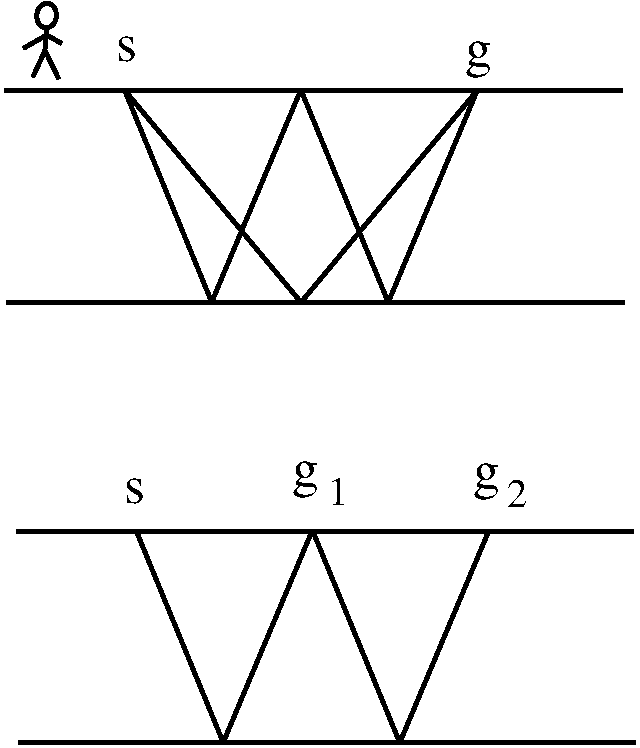
\includegraphics[width=0.65\textwidth]{mltp/multangle}
\caption[multangle]{到达恒定炮检距的射线具有各种不同角度,因而也就是具有各种不同Snell参
量(左图)。具有恒定Snell参量的射线到达时,可以有各种不同的炮检距(右
图),Snell参量p值恒定时,所有各个路程均有相同旅行时间
}
\label{fig:mltp/multangle}
\end{figure}

为了解野外资料是如何同倾斜叠加联系起来的,需从在共中心点道集上搜索那些在双曲
线波至达到某个特定鋇率值$p=dt/df$之处的所有能量开始说起,地面覌测资料上所见的这些
能量片断,每个都可告诉我们具有该Snell参量p的射线是在何处和何时到达地靣的,典型的
几何关系和合成数据如图\ref{fig:mltp/intervalvel1}和图\ref{fig:mltp/intvel2}所示。



\begin{figure}[H]
\centering
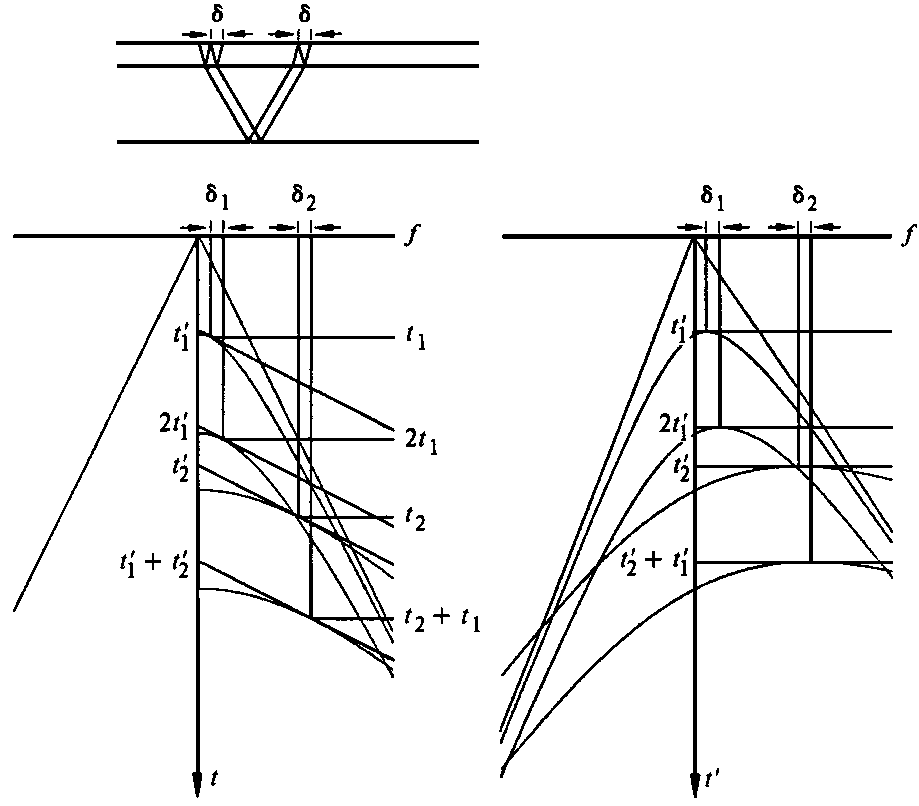
\includegraphics[width=0.65\textwidth]{mltp/intervalve1}
\caption[intervalve1]{表示同相轴$(t_1,2t_1,t_2,t_2+t_1)$的二层模型。
顶部图是射线路程,左图是通常的数据道集,右图是该道集经过线性时差校正$t'=t-pf$
之后重新显示的结果。各图系按比例为$(1,2,3)$的参量$(v_1,v_2,1/p)$计算出来。注意与斜率为p之直线相切处的
同相轴片断,我们看得出到达时间有垂直入射时的关系---就是说,混响周期是固定的。而且对微屈多次
波和对简单多次波都一样。之所以必然如此,是因为顶部的图中之射线路程可以精确地应用于那些在
出之处的同相轴片断;此外,由于$\delta_1=\delta_2$,时间$(t_1',2t_1',t_2',t_2'+t_1')$也是同熟悉的垂直入
射模式一样(据Gonzalez)
}
\label{fig:mltp/intervalve1}
\end{figure}

\begin{figure}[H]
\centering
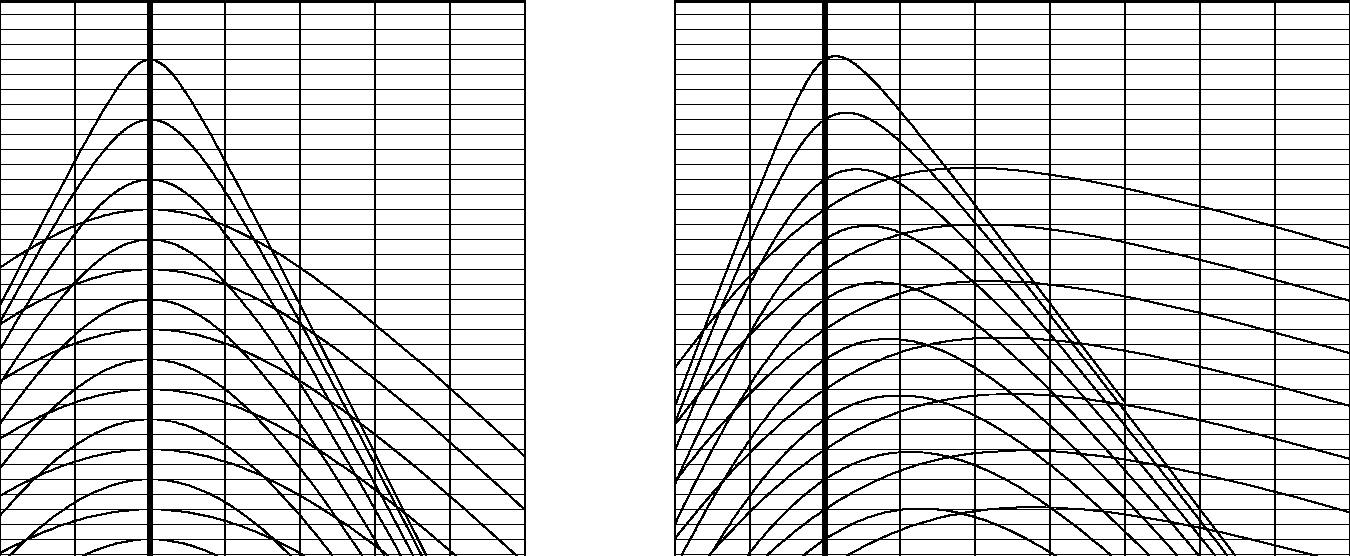
\includegraphics[width=0.65\textwidth]{mltp/intvel2}
\caption[intvel2]{
除表示出有更多多次反射之外,此图与图\ref{fig:mltp/intervalvel1}
是相同的
}
\label{fig:mltp/intvel2}
\end{figure}

$t_i$与$t_i'$二者的行为性质都像法线入射多次反射的时间。尽管任何能量片断之横向位置令
人遗憾地是与速度模型$v(z)$有关,可是进行倾斜叠加却无关于横向位置。原则上,可以用
许多离散的p值完成倾斜叠加,使$(f,t)$空间映射为$(p,t)$空间。利用$(p,t)$空间妙就妙
在多次波压制问题可以分解成许多单独的一维问题,每一个力值各相应于一个问题;不仅如
此,而且求解这些问题不需要已知地层速度,反倒轮到由你从已公布的许多方法中去挑选你
爱用的方法了。在压制多次波之后,你就作逆倾斜叠加,一旦变回至$(f,t)$空间,你就能
佶计速度并利用你拿手的叠加方法进一步压制多次波。

图\ref{fig:mltp/intvel2}是一种“工作手册”式的练习。把右图中所有同相轴的顶部挑出来,然后用虚
线把它们联起来,你就能够证实海底微屈多次波具有像简单樺底多次波一样的层速度。沉积
地层的层速度可由一次波测定出,将第n简单多次波与第n微屈多次波联起来也可以测定出沉
积地层的速度。

用反褶积方法消除交混回晌的办法坷利用倾斜叠加变换至一维问题情形来代替,例如,
可参阅Treitd等人的论文(1982
)。这是介于试验研究工作与工业生产实践二者之间的一
项矬理方法,有待进一步完善。它的强有力之处在于它既正确地掌握了固有的反射系数之角
度依赖关系,又正确地掌握了由炮点与检波点之几何分布形式所形成的角度依赖关系。它的
弱点之一是它假设产生混响的地层内具有横向均勻性,海水层倒是极均勻的,但是海底沉积
物却可能相当不均匀。

\subsection{近地表不均匀性}
\label{sec:5.6.2}

土壤层具有奇怪的声学性质,地震波在其中的传播速度一般小于或等于水中的声速1500
米/秒;土壤层的速度比水中声速低五倍、即像空气中的声速一样慢(
300米/秒),也并非
少见的事。实际工作时,地震震源均埋置于风化带之下。除了在沼泽地区外,接收器大多总
是必须置于风化带之上,在沼泽区的野外工作非常困难,以致你要比平常少用许多检波器。

非常困难的根源在于土壤层是显著横向不均匀的。两个相距不过10米的检波器得出很不
相同的地震记录,并不稀罕。尤其是,井口时间(由炮井底部至井顶附近地面的地震波旅行
时间)可以很容易显示出相当于整个波长的时间异常,尽管实际是平坦水平的地面,对风化
带内有如此明显而不可预测的旅行时间异常如何理解呢?这得用河流蛇曲、超浅层气藏、碳
酸盐岩溶洞、冰碛物等等的影响去解释,所有这些不规则性影响在深部虽也能发现,但是只
要含水饱和度和地下压力并未减小阻抗的非均匀性,那么在近地表处的那些不规则性影响就
更严重。关于这个问题尚可参阅\ref{sec:3.7}节的论述。

浅海情形要好一点,横向变化仍存在有充分机会---那里不但有埋藏的古河道而且还有
埋藏的海底水道,但是浅海情形的主要问题变成了海水层的鸣震问题,观测资料的功率谱将
受这种鸣震所控制。

与此情形类似,对陆地资料而言,功率谱总是逐个记录站而迅速变化的,谱的这些变化可
解释为多次反射之变化,而多次反射之变化则是由有效深度或风化带特征之变化所引起的。

\subsection{模拟时应注意之点}
\label{sec:5.6.3}



向下延拓方程包含四种主要因素:检波点处介质之慢度$1/v(g)$;炮点处介质之慢度
$1/v(s)$;炮检距空间内之时差$k_h/\omega$;中心点空间内之倾角$k_y/\omega$。这四种因素均具有相同
物理量纲,因而按照假设存在于各因素之间的数值不等式关系可以将模拟处理过程加以分
类。一维工作忽略四种因素中的三种,即倾角、时差和差值$v(g)^{-1}-v(s)^{-1}$。
共中心点叠
加包括时差$k_h/\omega$,关于是否包括倾角或横向速度变化,我们现在可以有选择的自由;横向速度
变化往往是在存在有微屈多次波的地表面附近十分显著;记住来自深部地下界面的典型情形
是射线以陡角度在低速地面出射这个简单概念,当在近地面处应兩延拓方程时,由于应有
$1/v>>k_y/\omega$,略去倾角是特别正确的。既然我们的野外工作极难控制超岀射线平面之外的倾
角,最好是找到这种可以略去倾角的借口
。另一方面,炮检距空间的时差大概总是在射线平
而之内要比在射线平面之外大很多。

对多次反射进行模拟或处理时,另一种重要因素是上行波与下行波的耦合作用。这种耦
合作用引进了在炮点下方的反射率$c(s)$和检波点下方的反射率$c(g)$。以后我们还会讨论的
一个重要可能性就是:纵使所有角度均能忽略,$c(s)$还是可能不同于$c(g)$。

\subsection{多次反射相减消去法}
\label{sec:5.6.4}

进行叠加可看作是加法过程,进行模拟则导至减法处理,该减法过程是对叠加的补充而
不是替换物:在相减之后,你就可叠加。

首先我们试图模拟该多次反射,然后我们试图从数据中把它减掉。一般而言,用减法消
除多次波比用加法消除多次波有更多危险。为成功地运用减法,不但要求时间误差小于四分
之一波长而且要求有正确的振幅。

为考虑说明模拟结果与现实之间的偏差,可引入以统计方法确定的经验常数。在统计学
中,这种方法以回归方法而知名。例如,已知数据点集合应拟合于某一直线时,我们即可对
残差利甩最小二乘法确定该直线的最佳参量。这样,移去该直线,就可以开始仔细研究这些
数据点了。这非常像我们打算进行的多次反射消除,如有可调参量自然可以更有助于考虑在
计算精确多次波振幅时可望遇到的困难。未知的时间误差非常难以模拟。因为存在有数学上
的非线性性质,有种稍微不同但更易于控制的办法,就是将褶积滤波中的系数取为可调参
量,这样一种滤波可以代表任何比例因子和时移。采用时变滤波来计算时变模拟误差,是引
人感兴趣的办法。采用这种办法时逃避不了的一个困难是:一项滤波因子可能代表一大堆东
西而不仅限于标定和振幅。你采用的参量越多,模型就将越能拟合于数据,不论该模型是否
真正地与数据有关。

将多次反射减去时所发生的困难实际上仅仅是这样:模拟多次波时---比方说,模拟其
几何分布或速度时---如果有不合适之处,这时你需要在回归方法中利用许多可调参量进行
适当的补偿,而采用很多可调参量,就不但减去了多次波而且还可能减掉了一次波,这真是
泼洗澡水连孩子也一块泼出去了!

\subsection{倾斜反褶积与反演}
\label{sec:5.6.5}

因为实际工作采用宽炮检距,事情已日益明显,地震学家必须逐个研究多次反射并注意
海底的差异。Taner (1980)曾介绍过一种可以如此作的直接而又吸引人的方法,那就是他
的径向记录道法(radial-trace method),径向记录道是沿恒定值$r=h/t$的某条直线斜穿
过共炮点道集的一条直线。我们不对恒定炮检距上的记录道进行反褶积,而对径向记录道采
用反褶积。反褶积可推广至向下延拓过程,径向记录道的向下延拓能用时移来近似。可惜,
当直线上的数据是由海底多次波和微屈多次波组成时会出现问题,因为这些多次波要求有不
同的轨线,以Snell波为工具是可以解决这个问题的,至少在原则上可以如此。Estevez
(1977)在其学位论文中从理论上证明了Snell波如何也能用于解决像绕射与横向速度变化
(如果已知)这类困难。Estevez的论文中有个阐明海底深度相异对不同多次反射有密切影响
的例子,如图\ref{fig:mltp/estevez}所示。

\begin{figure}[H]
\centering
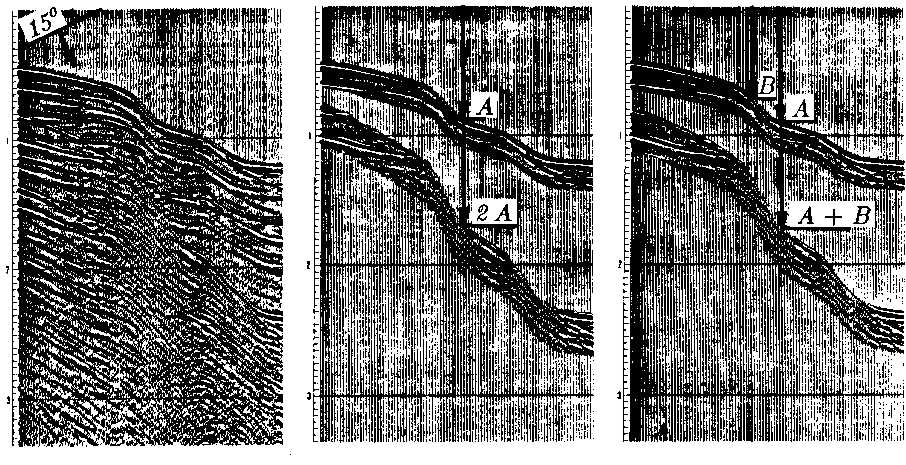
\includegraphics[width=0.65\textwidth]{mltp/estevez}
\caption[estevez]{
多次波之时间与所有时间之和有关(据Estevez )
}
\label{fig:mltp/estevez}
\end{figure}

大多数反演赴理所面临的问题都是由资料缺乏完整性引起的,资料可能是在时间和空间
方面或在它的谱方面不完整。对任何递归方法均须加以认真分析,以保证在浅层深度上所造
成的误差不至于在继续往下算时会不受控制地发生混合。一切资料在谱方面都是不完整的,
还有,利用一切资料时都有个关于爆炸波形的不确定性问题。在值受到微屈多次波的不利
影响时,第一个海底反射通常出现在过于靠近勘探船之处,严格来说是记录不到的。为解决
这个问题,Taner建立了一种特殊辅助记录系统。

Snell波方法有个好处,进行倾斜叠加就能由原始野外资料形成某种信噪比増强,但是
它也有个不利之处,向下延拓必须一直进行到所有深度。以后所要讨论的一些方法均属叠前
方法,不过它们并不要求向下延拓到低于海底。

\subsection{分裝法Backus滤波}
\label{sec:5.6.6}

为了处理地面多次反射,我们准备提出一种普遍性的策略、即阻抗置换方法.这种策略
将需要以回归理论和波场延拓理论作为重炮武器,为了不至于迷失目标,我们将用取自理想
化几何关系的一个例子来开始着手讨论。Larry
Morley曾以实例说明实际情况与这种理想
化精形相距并不太远,其博士学位论文(1982
)阐述了应用这种方法的一项成功试验并详细描述了阻抗置换的策略。

试想像海底是平坦的,取炮点附近的海底反射系数为$c_s$,在检波点附近则取为$c_g$,检波
点附近的混响模式为
\begin{equation}
\frac{1}{1+c_gZ}=1-c_gZ+c_g^2Z^2-c_g^3Z^3+c_g^4Z^4+......
\label{eq:ex5.6.1}
\end{equation}
式中,Z为传播至海水层底部情形下的双程延迟算子(见\ref{sec:4.
6}节或《地球物理数据处理基础》
一书关于Z变换背景的讨论)。在炮点附近有类似的混响序列:
\begin{equation}
\frac{1}{1+c_sZ}=1-c_sZ+c_s^2Z^2-c_s^3Z^3+c_s^4Z^4+......
\label{eq:ex5.6.2}
\end{equation}
忽略G与q之间的差别,则导至Backus混响序列,它是式\ref{eq:ex5.6.1}与式\ref{eq:ex5.6.2}的乘积。

\begin{equation}
\frac{1}{1+cZ}\frac{1}{1+cZ}=
1-2cZ+3c^2Z^2-4c^3Z^3+5c^4Z^4+......
\label{eq:ex5.6.3}
\end{equation}

式\ref{eq:ex5.6.3}左端的分母就是Backus滤波算子,采用这个滤波算子应可消除混响序列。
Morley将明显包含炮点与检波点之差异所形成的该种滤波算子称为分裂法Backus滤波。深
度以及反射系数均可能横向变动(倾角影晌是二阶量),于是分裂法Backus算子可取为:
\begin{equation}
(1+c_se^{i\omega\tau(s)})(1+c_ge^{i\omega\tau(g)})
\label{eq:ex5.6.4}
\end{equation}
求式\ref{eq:ex5.6.4}的倒数,将它展开成类似于式\ref{eq:ex5.6.3}的表达式,你就会发现第n项分裂成n个
项了,这正是意味着炮点附近海底反射的路程可以具有不同于检波点附近海底反射路程的旅
行时间。


下面的图\ref{fig:mltp/splitpeg}取自Morley的学位论文,它表明分岔的微屈多次波是一种可观察到的现
象。他对该图有下列解释:

该图系偏移距略小于电缆长度二分之一情形下取自同一测线的共炮检距剖面(COS
)(偏移距为45个炮点)。在左侧2.5秒时开始一直延续至右侧3秒时的一阶微屈多次波在近
记录道剖面上是“蜕化”的(未分岔),而在这个COS剖面上则由于受海底地形影响却是分
岔的,最大分岔出现在炮点180至200附近,约为200毫秒。正如人们所预料,这最大分岔出
现在海底具有最大倾角之处,即炮点位置与检波点位置上饰海底深度之差为最大之处。

\begin{figure}[H]
\centering
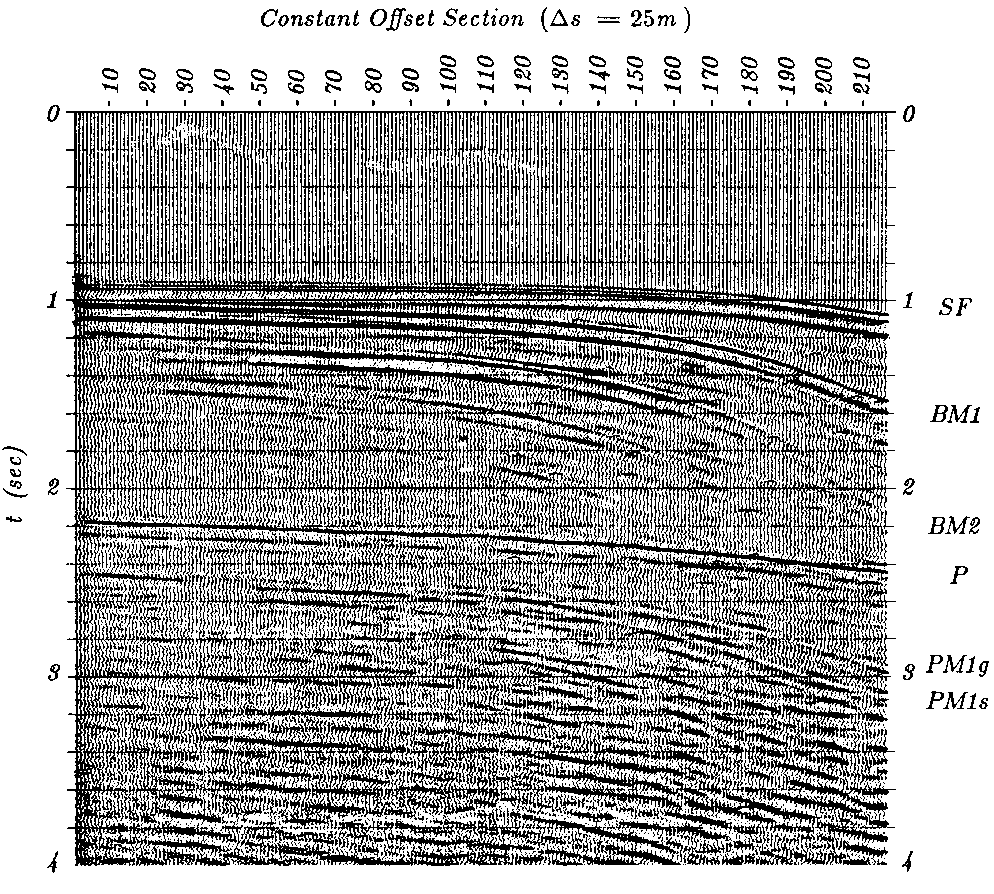
\includegraphics[width=0.65\textwidth]{mltp/splitpeg}
\caption[splitpeg]{
共炮检距剖面(COS),所在测线与\ref{sec:5.5}节中之图\ref{fig:mltp/nearoffset}的测线相同,偏移距
约为45个炮点距离.注意,一阶微屈多次波现在分岔成为两个明显可区别的波
至$PM_{1s}$和$PM_{1g}$ (据Morley )
}
\label{fig:mltp/splitpeg}
\end{figure}

目前大多数处理方法均完全忽略了Backus滤波而对每个地震记录道采用独立的反褶积
滤波求解办法,这种作法引入了大量自由参量,与此相比之下,分裂法Backus滤波处理办法
在保存一次波方面应能起比较好的作甩。

在实际应用时,我们预料任何以分裂法Backus滤波概念为基础的方法将需要包括时差校
正影响。很幸运,速度差异会减小微屈多次波的出射角。当然了,剩余时差问题会使海水层
底部多次波成为一种非常麻烦的事,在那种场合下,大概是应当在正常时差校正之后才能应
用该种处理。以下让我们考察一下对分裂法Backus算子作估计的问题。

\subsection{海底一致性多次波压制}
\label{sec:5.6.7}

长期以来都是采用所谓地面一致性静校正模型(surface-consistenstatics model)处
理不规则时移问题,采用这种模型时,你是将所观测时移$t(s,g)$
拟合于一种回归模型$t(s,g)\approx t_s(s)+t_g(g)$,
以统计方法确定的函数$t_s(s)$和$t_g(g)$可以解释为是根据
直接位于炮点与检波点之下的高程或速度变化所导出的函数。Taner与Coburn (
1980 )曾介
绍过一种与此密切相关的地面一致性频率响应模型概念作为静校正问题的一部分,我们将对
这种处理办法加以解释和推广。对于数据$P(s,g,\omega)$,我们的直观模型是
\begin{equation}
P(s,g,\omega)\approx \frac{1}{1+c_se^{i\omega\tau(s)}}
\frac{1}{1+c_ge^{i\omega\tau(g)}}e^{\frac{i\omega}{v}\sqrt{z^2+4h^2}}
H(h,\omega)Y(y,\omega)F(\omega)
\label{eq:ex5.6.5}
\end{equation}
其中,头两个四子代表分裂法Backus滤波;其次的因子代表正常时差校正;因子$Y(y,\omega)$
是中心点y以下的与深度有关之地层模型;因子$H(h,\omega)$是剩余时差;最后的因子$F(\omega)$
是由地层与记录系统二者形成的某种平均滤波。

与分裂法Backus滤波有关的一个很熟悉的问题是,时同延迟$\tau(s)$与$\tau(g)$是以非线性方式引入该模型的。所以使它线性化后,可将该模型推广为
\begin{equation}
P'(s,g,\omega)\approx S(s,\omega)G(g,\omega)H(h,\omega)Y(y,\omega)F(\omega)
\label{eq:ex5.6.6}
\end{equation}
现在,S含有炮点位置上的所有海水层混响影响特征,包括汽枪本身的任何不规则表现在
内;与此类似,接收点的各种影响均包含在G内;对P已经作过时差校正,因而也就限定了
$P'$。

从理论上说,取其对数即得出一种线性可加性模型:
\begin{equation}
lnP'(s,g,\omega)\approx lnS(s,\omega)+
lnG(g,\omega)+lnH(h,\omega)+lnY(y,\omega)+lnF(\omega)
\label{eq:ex5.6.7}
\end{equation}

$P'$的相位,即该对数之虚部,包含着数据内之旅行时间信息,当数据是由一个以上的
波至所构成时,这种信息就开始丧失其意义,即使数据的质量良好,相位函数也变成不连续
的了。因此,在实际应用时是把注意力限制于式\ref{eq:ex5.6.7}的实部,它实际上就是关于功率
谱之表述。如式\ref{eq:ex5.6.7}所示的分解,是一个线性问题,或许用叠代方法求解才最好,因
为问题涉及到高维数。在根据功率谱重建S与G时,Morley利用了Wiener-Levinson算
法,为计及在海水层中的路程,在滤波因子S与G中直接令时间域置零。他略去了式\ref{eq:ex5.6.5}
中明显的时差校正项,这样就能照顾到他仅仅利用排列内半侧的事实


\subsection{多次波压制方法之置换介质概念}
\label{sec:5.6.8}

在地震学中,地震波波长往往都很长,促使我们忘记了在物理上还可能存在有定向波动
源和定向接收这码事。假设我们已经有了、或以某种方式模拟出了仅向下辐射的震源和仅接
收上行波之接收器;接着再假设,我们己经能够以某种方式把这科震濾和接收器向卞延拓到
海底之下。这样就将能消除掉广泛一类的多次反射,海底多次波和微屈多次波将消失。达到
那样的结果可算是一种重要成就了。不过,还有一个次要问题尚留待解决,数据资料现在也
许是沿一条不平坦的、但随海底地形而起伏的测线分布,因此还要作最后一步的处理,这一
步很容易作,就是要通过某种没有强烈而又混杂的海底反射系数之替代介质向上延拓。以上
所述处理过程将称作阻抗置换,它类似于在重力数据换算中利用替代介质,也类似于以某种
置换速度(replacement velocity)使地震记录出现时移(见\ref{sec:3.7}节)。

偏移运算是将上行波向下延拓,阻抗置换这种运算则像是将一条只能接收上行波的检波
点测线向下延拓。在现实情形中,埋置的各检波器既见有上行波也见有下行波。震源或接收
器之方向性表现在用于波场外推的平方根方程所选之符号上。根据互换原理,也可以将炮点
向下延拓。与此类似,从物理上说,炮点既向上也向下辐射能量,但是我们可将炮点想像成
是向上辐射或向下辐射,从数学上说,这不过就是一个符号选择问题。因此,在海底处的四
种可能观测排列所得结果以及上行与下行定向炮点和定向接收器的所有可能性,均可据此推
演出来。

将所有这种信息通过海底边界面进行外推时,要求估计出海底反射系数,这个系数是在
将海底以上各种波构成线性组合时作为比例因子参与计算的,进行反射系数估计所隐含的思
想可用数学上是等价的两种方式加以表达:
\begin{enumerate}
\item 从上方或下方入射到海底边界面的各种波应有在零延迟时间上等于零值的互相关
函数;
\item 从下方入射在该边界面的波应有极小功率。
\end{enumerate}

在检波点低于海底以后,你必须开始着手考虑使炮点低于海底。为求助于互换性原理,
有必要使炮点与接收点的方向性颠倒反转,这就是为什么需要在处理过程中包括有上行指向
之炮点与接收点的辅助观测排列的原因。

\subsection{习 题}
\label{sec:5.6.9}

\begin{enumerate}
\item 参阅图\ref{fig:mltp/intvel2},回答下列问题:
\begin{enumerate}
\item
  何种图解测定法可证明简单海底多次波之层速度等于微屈多次波之层速度?
\item
  何种图解测定法可确定沉积层之速度?
\item
  参照海水层之速度,试推演出Snell参量p的数值。
\item
  试导出沉积层之速度对海水层之速度的数值比
\end{enumerate}
\item   试考虑已知各层阻抗为$(I_1,I_2,I_3,...)$的某种成层介质上所观测到的上行波U,
  以及在阻抗为$(I_1,I_2,I_3,...)$的介质之表面上的上行波U',注意其中顶部的地层阻抗
  已改为$I_2$。
  \begin{enumerate}
  \item
  试画出某些多次反射的射线路程,它们均应只存在于第一种介质内,而不应存在于
  第二种介质内。
\item
  假设你能找到一种数学处理万法可将波场U转换为波场U',试问从U'中消除的什
  么多次波将是不能用Backus算子来消除的?
\item
  试利用《地球物理数据处理基础》一书第8章中所述方法,导出以U、$I_1$和$I_2$表示
  的一个关于$U'$之方程,其中不得涉及$I_3$、$I_4$、...
  \end{enumerate}
\end{enumerate}